\documentclass[10pt,twocolumn]{article}

% Two typographic variants share one body.  Build the default Times look with
%   make
% and the Latin Modern (Computer Modern) look with
%   make lmodern
% which sets \paperstyle before this file is read.
\providecommand{\paperstyle}{times}
\input{paper/style-\paperstyle}

\newcommand{\gparity}{\textsc{G1}}
\newcommand{\rnse}{\textsc{rnse}}
\newcommand{\infb}{\mathrm{INF}_{B}}
\newcommand{\method}[1]{\textsc{#1}}

\input{paper/titleblock-\paperstyle}

\begin{document}
\maketitle
\vspace{-1.2em}

\begin{abstract}
\noindent
Hand-constructed transformers provide unusually strong ground truth: their
forward pass, intermediate state, and intended circuit are known exactly.
This does not imply that gradient descent can recover the same computation,
even when the constructed solution belongs to the trainable model's
hypothesis class. We study this prerequisite using a weight-tied transformer
whose forward pass executes Bellman--Ford relaxation. The construction is not
our novelty; its useful properties are exact verification, complete per-round
state, and exact embedding into a trainable twin. On directed graphs with at
most four nodes, a widened, LayerNorm-free, weight-tied model trained from
random initialization reaches 96.97\% held-out graph exactness, 98.85\% node
exactness, and 96.97\% exactness on reachable non-source nodes. The embedded
construction attains 100\% exactness, zero objective, and zero gradient, yet
the learned endpoint remains approximately as far from the constructed
parameters as initialization. A matched short run is still improving at
50.20\% graph exactness, while an 80,000-step run saturates near 97\%.
Perturbation experiments support optimizer-step drift rather than an
objective that rewards loss of exactness. These are single-seed,
small-graph diagnostics. We do not run the tied-versus-untied experiment
needed to determine whether recurrence causes learned relaxation.
\end{abstract}

\vspace{0.3em}
\noindent\textbf{Keywords:} algorithmic transformers, Bellman--Ford,
weight tying, optimization, mechanistic interpretability

\section{Introduction}

Neural algorithmic reasoning asks whether a model has fit an input--output
relation or learned a procedure that remains valid outside the training
distribution. Shortest paths make the distinction concrete. A model can
implement repeated local relaxation, exploit a correlated graph statistic,
memorize a bounded-size mapping, or compute a different but behaviorally
adequate algorithm. In-distribution output accuracy does not identify which
explanation is correct.

Prior work establishes both sides of this problem. Shallow transformers can
learn shortcut implementations of formal languages that fail under
distribution shift \citep{liu2022shortcuts}. A trained shortest-path
transformer has been reported to use spectral navigation rather than textbook
dynamic programming \citep{cohen2025spectral}. Conversely, recurrent
transformers can learn iterative procedures with length generalization
\citep{fan2024looped}, and sparsity-regularized graph neural networks can
recover Bellman--Ford-like relaxation \citep{nerem2026gnn}. The broad claim
that trained models always fail to learn algorithms is therefore both
occupied and false.

A controlled comparison needs a prerequisite stronger than ordinary task
accuracy: the intended solution must be present in the trainable hypothesis
class. Otherwise, failure to learn the intended circuit is uninterpretable.
We call this requirement \textbf{\gparity{} parity}. A trainable model has
\gparity{} parity when the hand-constructed parameters load into it and
reproduce exact outputs and zero objective. This test rejects apparently minor
architectural changes---most notably LayerNorm here---that alter the literal
arithmetic performed by the construction.

This paper reports the diagnostic work required to establish \gparity{} parity
and learnability in one model family. Its contributions are deliberately
bounded:

\begin{enumerate}
  \item We present an exact Bellman--Ford transformer as executable
  optimization ground truth. The construction follows existing expressivity
  work; the contribution is the bit-exact verifier, complete round state, and
  direct embedding into a trainable twin.
  \item For one seed and graphs with at most four nodes, a \gparity-compatible
  model learns near-exact behavior from random initialization. This separates
  representability from the optimization failure observed in shorter runs.
  \item We characterize local drift around the exact circuit. The construction
  is a zero-loss, zero-gradient global minimum, and learning-rate-controlled
  runs recover exact behavior without recovering the original parameters.
\end{enumerate}

The claim boundary is central. We do \emph{not} show that weight tying makes a
trained transformer use Bellman--Ford relaxation. We did not run an untied
comparator, size extrapolation, state probes, attention comparison, iteration
ablation, or causal intervention. Those are requirements for a later
mechanistic experiment, not results of this study.

\section{Related Work}

\subsection{Compiled and looped transformers}

RASP provides a programming abstraction for transformer computation
\citep{weiss2021rasp}. Tracr compiles restricted programs into transformer
weights, producing models with known internal structure
\citep{lindner2023tracr}. Looped-transformer constructions show that a reused
block can implement iterative programs \citep{giannou2023looped}. Most
directly, \citet{deluca2024simulation} construct looped transformers for graph
algorithms and discuss finite-precision and softmax limitations. These works
preclude a construction-novelty claim for our model.

Our distinction is engineering and measurement discipline. The artifact
exposes all residual registers after every relaxation, supplies an executable
Bellman--Ford reference trajectory, and is tested for exact agreement rather
than approximate task accuracy. The same parameter tensors embed into a
widened trainable module with all added coordinates set to zero.

The implementation uses two different exactness mechanisms. Pairwise minima
use the identity
\begin{equation}
  \min(a,b)=a-\operatorname{ReLU}(a-b).
  \label{eq:relu-min}
\end{equation}
Routing uses a fixed float32 score gap large enough that non-target
exponentials underflow to zero. The latter is an implementation property
dependent on dtype and kernel behavior, not exact hard selection by
finite-logit real-arithmetic softmax. Approximate sharpness of ordinary
softmax requires score spread growing with set size and desired error
\citep{velickovic2025softmax}.

\subsection{Learned algorithms and shortcuts}

\citet{liu2022shortcuts} show that low-depth transformers can fit automata
through shortcuts that fail outside the training regime. On graphs,
\citet{cohen2025spectral} analyze a trained shortest-path transformer and
report a spectral mechanism rather than Bellman--Ford or Dijkstra-style
dynamic programming. These results own the broad shortcut-learning headline.

The negative conclusion is not universal. Looped transformers have been
trained to learn iterative solutions with length generalization
\citep{fan2024looped}. Sparsity-regularized GNNs can recover a fixed number of
Bellman--Ford iterations and extrapolate to larger graphs
\citep{nerem2026gnn}. MINAR recovers compact Bellman--Ford-like circuitry in a
trained GNN and also demonstrates that correct outputs can conceal an
unintended internal shortcut \citep{he2026minar}.

The remaining narrow question is whether weight-tied recurrence changes what a
trained transformer learns when an exact relaxation circuit exists in the
same architecture. The present study validates a prerequisite for asking that
question, but does not answer it.

\subsection{Known-circuit interpretability}

InterpBench argues that mechanistic-interpretability methods need models with
known circuits beyond raw Tracr programs \citep{gupta2024interpbench}. A
hand-constructed graph algorithm offers exact labels at the level of registers
and iterations, but one model is not itself a benchmark. Establishing
benchmark value would require comparing interpretability methods or exposing
a specific failure against the known circuit.

Intermediate-state probes would also be insufficient alone. Candidate
algorithmic state can be decodable without being causally used
\citep{darade2026represented}. A future claim that a trained model executes
relaxation must therefore combine state alignment with interventions.

\section{Exact Transformer Artifact}

\subsection{Algorithm and state}

For source \(s\), Bellman--Ford initializes
\begin{equation}
  d_s^{(0)}=0,\qquad d_v^{(0)}=\infb\quad(v\ne s),
\end{equation}
where \(\infb=N_{\max}W_{\max}+1\) exceeds every representable simple-path
length. Each round computes
\begin{equation}
  d_v^{(t+1)}
  =
  \min\!\left[
    d_v^{(t)},
    \min_{(u,v,w)\in E}\left(d_u^{(t)}+w\right)
  \right].
  \label{eq:bf}
\end{equation}

The sequence contains one sink token, a fixed allocation of node tokens, and a
fixed allocation of directed-edge tokens. Residual coordinates encode node
identities, the distance register, edge endpoints and weights, candidate
slots, and temporary routing state. A single block performs one relaxation (Figure~\ref{fig:architecture}):
edge tokens read source-node distance; gather heads route incoming candidates
to destination slots; a ReLU network folds those candidates with the previous
distance; and a residual delta writes the result while clearing scratch state.
The same block is reused \(N_{\max}-1\) times. An optional extra round detects
a reachable negative cycle by checking whether a distance decreases.

\begin{figure*}[!t]
\centering
\begin{tikzpicture}[
  node distance=0.55cm,
  >=Latex,
  block/.style={
    draw=navy, rounded corners=2pt, very thick,
    fill=lightblue, minimum height=0.72cm, text width=2.15cm,
    align=center, font=\small
  },
  state/.style={
    draw=darkgray, rounded corners=2pt, thick,
    fill=lightgray, minimum height=0.72cm, text width=1.65cm,
    align=center, font=\small
  },
  arrow/.style={->,thick,color=darkgray}
]
\node[state] (tokens) {Sink, node,\\edge tokens};
\node[block, right=of tokens] (read) {Source read\\attention};
\node[block, right=of read] (gather) {Destination\\candidate gather};
\node[block, right=of gather] (min) {Exact ReLU\\minimum fold};
\node[block, right=of min] (write) {Distance writeback\\and cleanup};
\node[state, right=of write] (next) {Next-round\\residual state};
\draw[arrow] (tokens) -- (read);
\draw[arrow] (read) -- (gather);
\draw[arrow] (gather) -- (min);
\draw[arrow] (min) -- (write);
\draw[arrow] (write) -- (next);
\draw[arrow,rounded corners=5pt] (next.south) -- ++(0,-0.38) -|
  node[pos=0.48,below,font=\footnotesize] {same parameters, repeated \(N_{\max}-1\) times}
  (read.south);
\node[draw=accentred,dashed,rounded corners=2pt,fit=(read)(gather)(min)(write),
  inner sep=5pt,label={[font=\footnotesize\color{accentred}]above:one weight-tied relaxation block}] {};
\end{tikzpicture}
\caption{The constructed residual program. Attention performs fixed routing;
the ReLU fold performs exact arithmetic minimum; the full block is reused for
each Bellman--Ford round.}
\label{fig:architecture}
\end{figure*}

\subsection{Verification and tracing}

The verifier independently computes every Bellman--Ford reference state.
Integer-weight outputs are bit-exact against NetworkX's single-source
Bellman--Ford implementation; a seeded 1,000-graph property suite spans graph
sizes through the configured maximum. The tracer records the full residual
stream, named sublayer deltas, and attention patterns.

This verification does not make the construction novel. It makes the
construction an exact reference point for optimization and later mechanistic
comparison.

\section{Trainable Twin and \gparity{} Parity}

The trainable twin preserves tokenization, residual-register layout, sublayer
order, head topology, and recurrent application. Attention projections and MLP
hidden spaces may be widened. To load the construction, each original matrix
is copied into the leading block of the wider tensor and every additional
entry is set to zero. Widening therefore preserves the exact constructed
function.

LayerNorm is optional in diagnostic variants but incompatible with \gparity{}
parity: normalizing the residual stream rescales literal distances. A
\gparity{} audit requires a LayerNorm-free model, an exact constructed-weight
load, exact decoded outputs, and zero objective.

The widened LayerNorm-free model passes this audit. Validation and test graph,
node, reachability, and reachable-non-source exactness are all 100\%;
supervised loss and MAE are zero; the full-objective gradient has zero
\(\ell_2\) norm and zero maximum absolute component; and Euclidean distance
from the constructed reference is zero. Since the objective is non-negative,
zero objective certifies that the construction is a global minimum of the
measured loss.

\section{Diagnostic Protocol}

All results are diagnostic. Completed runs use model seed 17 and data seed
20260730; the fixed validation and test sets contain 512 and 1,024 graphs.
Training graphs are freshly sampled on every batch. Graphs are directed, have
integer non-negative edge weights, and contain two to four nodes. The model
executes three tied rounds.

The principal random-initialization recipe uses width 128 for every attention
and MLP subspace, no LayerNorm, per-round supervision, batch size 128, and
Xavier initialization with gain 0.1. Optimization uses AdamW with
\(\beta=(0.9,0.999)\), zero weight decay, and gradient norm clipped to 1. The
learning rate warms up for 200 steps to \(3\times10^{-4}\), then decays by a
cosine schedule to zero over 80,000 steps.

\subsection{Objective and exactness}

The objective is mean Smooth-L1 loss over valid nodes and supervised rounds:
\begin{equation}
 \mathcal{L}
 =
 \operatorname{mean}
 \operatorname{SmoothL1}_{\beta=0.01}
 \left(\hat d/\infb,\ d/\infb\right).
 \label{eq:loss}
\end{equation}
For finite targets, a node is exact if
\(\lvert\hat d-d\rvert<0.5\). For unreachable targets, it is exact if
\(\hat d\ge\infb-0.5\). Graph exactness requires every real node to be exact.
We additionally report node exactness, reachability accuracy, and reachable
non-source exactness (\rnse). \rnse{} removes source and unreachable nodes,
the cases already correct under identity-like initialization.

\subsection{Saturation criterion}

No inherited accuracy threshold defines competence. A run is saturated only
if its terminal learning rate is zero and graph exactness, node exactness, and
\rnse{} each satisfy three conditions over the final two 10,000-step windows:
(i) final-window best improves by less than one percentage point over the
preceding window; (ii) absolute least-squares slope is below one point per
10,000 steps; and (iii) final-window range is below two points. This establishes
a measured plateau, not global optimality.

\subsection{Local perturbation diagnostic}

To separate loss--metric conflict from optimizer drift, we start from the exact
constructed parameters plus independent Gaussian noise with standard
deviation \(4\times10^{-4}\). These runs use the constructed-minimal, tied,
LayerNorm-free model. We measure objective and gradient at the construction,
then log validation loss, exactness, and Euclidean parameter distance.
Peak learning rates \(3\times10^{-5}\) and \(10^{-5}\) both decay to zero.

\section{Results}

\subsection{\texorpdfstring{\gparity-compatible training succeeds at
\(n\le4\)}{G1-compatible training succeeds at n <= 4}}

Table~\ref{tab:saturated} reports the saturated random-initialization runs. The
LayerNorm-free model reaches 96.97\% held-out graph exactness and 96.97\%
\rnse{}. This establishes a trainable, \gparity-compatible recipe in the
tested regime. LayerNorm is not necessary under the widened, long-horizon
recipe. The 0.78-point validation graph difference is a single-seed
observation, not an estimate of a systematic normalization effect.

\begin{table*}[t]
\centering
\caption{Saturated random-initialization runs. Exactness values are
percentages. The test reachability accuracy is 100\% for both runs.}
\label{tab:saturated}
\small
\begin{tabular}{lccccc}
\toprule
Architecture & \gparity{} & Best step &
Validation graph / node / \rnse{} &
Test graph / node / \rnse{} & Verdict \\
\midrule
Width 128, pre-LayerNorm & no & 70k &
\textbf{97.46 / 99.14 / 97.64} &
96.97 / \textbf{98.92} / 97.14 & saturated \\
Width 128, no LayerNorm & yes & 80k &
96.68 / 98.74 / 96.56 &
\textbf{96.97} / 98.85 / \textbf{96.97} & saturated \\
\bottomrule
\end{tabular}
\end{table*}

\begin{figure*}[t]
\centering
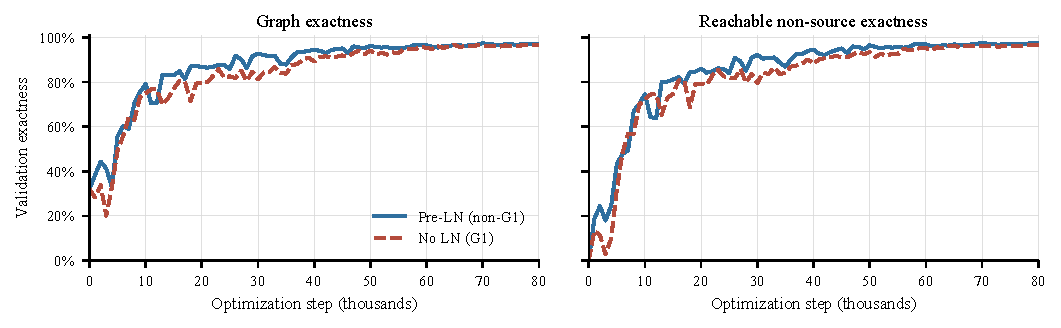
\includegraphics[width=0.97\textwidth]{paper/figures/saturation-curves.pdf}
\caption{Validation histories, logged every 1,000 optimization steps, from the
frozen v4 artifact.
Both width-128 models continue improving well past the original 4,000-step
budget. The no-LayerNorm run preserves \gparity{} parity.}
\label{fig:curves}
\end{figure*}

The trained no-LayerNorm endpoint is functionally successful but does not
approach the constructed vector. Its Euclidean distance from the construction
is approximately 76,648, versus approximately 76,649 at initialization. The
evidence establishes functional learnability, not literal recovery of the
known parameterization.

\subsection{The matched short run is budget-limited}

Table~\ref{tab:budget} compares otherwise matched LayerNorm runs. The
4,000-step condition ends at its best checkpoint and is not a ceiling.
Extending the schedule to 80,000 steps changes validation graph exactness by
47.27 points.

\begin{table}[t]
\centering
\caption{Matched training-horizon intervention.}
\label{tab:budget}
\small
\begin{tabular}{rrrrl}
\toprule
Steps & Graph & Node & \rnse{} & Curve \\
\midrule
4k  & 50.20 & 65.25 & 27.72 & improving \\
80k & 97.46 & 99.14 & 97.64 & saturated \\
\bottomrule
\end{tabular}
\end{table}

This intervention could have falsified a budget effect under the selected
recipe and instead found a large one. It does not show that duration was the
sole cause of earlier failure. The 4,000-step diagnostic already exceeds the
earlier approximately 18\% post-initialization graph exactness, so another
difference also mattered. Fresh versus fixed data, width 128 versus
constructed-minimal width, per-round versus final-only supervision, and batch
128 versus batch 32 remain untested as isolated causes.

\subsection{Drift is consistent with optimizer step size}

At the exact construction, the objective and both reported gradient norms are
zero. The loss therefore does not locally push the exact circuit away. After
perturbation, both zero-floor schedules recover exact or nearly exact behavior
(Table~\ref{tab:drift}). The smaller peak learning rate ends at 100\%
validation and test graph exactness, although parameter distance grows
slightly instead of returning to zero.

\begin{table}[t]
\centering
\caption{Constructed-basin perturbation diagnostics.}
\label{tab:drift}
\small
\begin{tabular}{rrrr}
\toprule
Peak LR & Val. graph & Test graph & Distance \(i\to f\) \\
\midrule
\(3{\times}10^{-5}\) & 100.00 & 99.80 & \(0.0355\to0.1257\) \\
\(1{\times}10^{-5}\) & 100.00 & 100.00 & \(0.0355\to0.0433\) \\
\bottomrule
\end{tabular}
\vspace{2pt}

\footnotesize Final losses are \(7.06{\times}10^{-7}\) and
\(7.58{\times}10^{-8}\), respectively; the construction has loss zero.
\end{table}

Across both logged trajectories, there are zero evaluation intervals in which
validation graph exactness falls while validation loss also falls. Exactness
declines coincide with higher validation loss, not an objective improvement.
Both endpoints have positive loss; the construction has zero.

These measurements support an ordinary optimizer-step explanation for the
previous drift: updates can leave a narrow exact region, and reducing peak
learning rate limits that movement. They do not support the alternative claim
that the regression objective rewards sacrificing half-unit-bin exactness.
Parameters need not return to the construction to recover the measured
function.

\section{Discussion}

\subsection{Representability is executable}

It is easy to describe a model as having ``failed to learn the known
algorithm'' when the intended circuit cannot be represented by the training
architecture. \gparity{} parity turns that ambiguity into a test: load the
construction, verify exact outputs, and verify zero objective. LayerNorm fails
because it changes the arithmetic state. Widening passes when the original
matrices are embedded and all new coordinates are zeroed. This is a practical
compromise: optimization is not restricted to constructed-minimal width, but
the exact circuit remains in the hypothesis class.

\subsection{Functional success is not circuit recovery}

The random model learns a near-exact function while remaining almost as far
from the constructed vector as at initialization. Local perturbation runs
recover exact outputs without returning to the reference parameters. Raw
parameter distance is therefore not a valid circuit-correspondence criterion
here.

This observation does not establish that the learned mechanism differs from
Bellman--Ford. Neural parameterizations have symmetries and redundant
representations, while widening adds alternative subspaces. Mechanistic
correspondence must be tested at the level of round state, routing,
intervention response, and executed function.

\subsection{What is known about failed short runs}

The supported causal claim is narrow: under the selected recipe, 4,000 steps
are insufficient and 80,000 steps reach saturation. The evidence does not show
that data reuse, minimal capacity, missing LayerNorm, supervision, or batch
size caused a prior failure. Those explanations remain hypotheses because the
corresponding one-factor interventions were not completed.

The distinction is methodological. A checkpoint at the end of an improving
curve supports ``budget-limited,'' not ``unlearnable.'' Conversely, a high
score under a favorable recipe does not identify which ingredient repaired an
earlier run.

\section{Limitations and Claim Boundary}

The limitations determine the contribution:
\begin{itemize}
  \item All completed training results use one model seed. There are no seed
  variances, confidence intervals, or population-level comparisons.
  \item Training and evaluation stop at \(n\le4\). An \(n\le8\) saturation run
  was not completed, and no graph-size extrapolation was evaluated.
  \item The principal recipe uses per-round supervision, fresh graphs, width
  128, batch 128, and 80,000 steps. Most ingredients were not isolated.
  \item The tied-versus-untied and final-only-versus-per-round grid was not run.
  Nothing here determines whether recurrence changes the learned mechanism.
  \item No probe matrix, shuffled-label baseline, attention agreement,
  iteration ablation, or causal state intervention was run.
  \item Parameter distance depends on parameterization, symmetries, and
  widening. It rejects literal vector recovery, not functional equivalence.
  \item Exact attention depends on tested float32 underflow behavior and is
  not a real-arithmetic softmax theorem.
  \item Saturation describes measured final windows; it does not prove that no
  better optimizer or longer schedule could improve the result.
  \item These diagnostics followed earlier failed pilots and are not a
  preregistered confirmatory experiment.
\end{itemize}

This is workshop-scale evidence for experimental validity and optimization
behavior. It is not a shortest-path generalization result and not a
mechanistic claim about learned relaxation.

\section{Deferred Mechanistic Experiment}

The exact artifact makes a stronger study possible, but that study remains
future work. A valid test must first reproduce \gparity-compatible
learnability at the intended \(N_{\max}=16\) scale, train on \(n\le8\), and
evaluate through \(n=16\). It would then compare tied and untied models under
final-only and per-round supervision across multiple seeds.

The decisive measurements are: (i) behavioral exactness stratified by size and
shortest-path hop count; (ii) a full \(k\times j\) matrix probing loop state at
iteration \(k\) for Bellman--Ford state after round \(j\), with random and
shuffled-label baselines; (iii) attention-routing agreement with the
construction; (iv) iteration ablation; and (v) causal interventions on decoded
round state, performed only if a probe diagonal appears.

Without these conditions, the question ``does weight-tied recurrence make a
trained model learn relaxation?'' remains unanswered.

\section{Conclusion}

An exact algorithmic transformer supplies more than an expressivity example:
it gives an executable global minimum, exact intermediate state, and a direct
test of whether a trainable architecture contains the intended solution.

In the small-graph regime, a widened, LayerNorm-free, weight-tied model that
contains the exact Bellman--Ford circuit reaches 96.97\% held-out graph
exactness from random initialization. The trained parameters do not recover
the construction. Local perturbation experiments show that exact functional
recovery depends on optimizer step size while remaining compatible with
parameter drift.

This resolves an experimental-validity objection, not the motivating
mechanistic question. Whether recurrence changes a trained transformer's
algorithm remains open because the required comparison was not run.

\section*{Reproducibility}

\begingroup\raggedright
Complete evaluation histories are frozen in
\path{docs/pilot-v4-curves.json}; the audit trail is in
\path{docs/pilot-v4-results.md}. Diagnostic implementation is in
\path{train/v3_model.py}, \path{train/v3_diagnostic.py}, and
\path{train/v4_diagnostic.py}. Source commit \texttt{6489e31} contains the v4
diagnostics; \texttt{ccb199b} freezes the report and curves. Runs used Python
3.11.9, PyTorch 2.11.0+cu126, and an NVIDIA RTX 3090.
\par\endgroup

\bibliographystyle{unsrtnat}
\bibliography{paper/references}

\appendix
\section{Evidence Ledger}

Table~\ref{tab:ledger} separates supported conclusions from unresolved causes.
This ledger is part of the claim boundary, not a list of proposed explanations.

\begin{table*}[t]
\centering
\caption{Evidence ledger. ``Untested'' means no causal conclusion is drawn.}
\label{tab:ledger}
\small
\begin{tabularx}{\textwidth}{>{\raggedright\arraybackslash}p{0.20\textwidth}>{\raggedright\arraybackslash}p{0.15\textwidth}>{\raggedright\arraybackslash}X}
\toprule
Question & Status & Evidence \\
\midrule
Does the trainable no-LN model contain the exact circuit? &
Established &
Constructed embedding gives 100\% exactness, zero objective, zero gradient,
and zero parameter distance. \\
Can that architecture train from random initialization at \(n\le4\)? &
Established for one seed &
Saturated held-out graph exactness is 96.97\%; held-out \rnse{} is 96.97\%. \\
Is LayerNorm necessary under the selected recipe? &
No, for one seed &
The no-LN run saturates within 0.78 validation graph points of pre-LN and ties
its test graph exactness. \\
Does training duration matter under the selected recipe? &
Established &
The matched 4k run is still improving at 50.20\%; the 80k run saturates at
97.46\% validation graph exactness. \\
Why did the original short pilot fail? &
Unresolved &
Budget matters, but the matched 4k diagnostic already exceeds the earlier
result. Fixed data, minimal width, final-only supervision, and batch size were
not isolated. \\
Does descent prefer lower loss at worse exactness? &
Not supported &
The construction has zero loss and gradient. No logged interval shows
validation loss and exactness falling together. \\
Does training recover the constructed parameters? &
No literal recovery &
The random endpoint remains approximately as far from the constructed vector
as initialization; local exact recovery also ends at nonzero distance. \\
Does weight tying cause learned relaxation? &
Unanswered &
No untied comparator, size extrapolation, probe matrix, iteration ablation, or
causal intervention was run. \\
\bottomrule
\end{tabularx}
\end{table*}

\section{Additional Completed Runs}

The primary text reports the two saturated width-128 endpoints and the matched
budget intervention. Table~\ref{tab:additional} records the remaining
completed random-initialization search. The 60k width-128,
\(3\times10^{-4}\) run is explicitly budget-limited because graph and \rnse{}
late-window gains exceed the saturation bound. Width 256 saturates below width
128 for this seed, falsifying the simple claim that additional width
monotonically repairs optimization. The \(10^{-3}\) run is also budget-limited
at 60k and therefore does not establish a lower asymptotic ceiling.

\begin{table}[ht]
\centering
\caption{Additional random-initialization diagnostics. Values are best
validation graph exactness / \rnse{}.}
\label{tab:additional}
\small
\begin{tabular}{rrrrl}
\toprule
Width & LN & LR & Horizon & Graph / \rnse{} \\
\midrule
128 & yes & \(3{\times}10^{-4}\) & 60k & 96.48 / 96.20 \\
128 & yes & \(3{\times}10^{-4}\) & 80k & 97.46 / 97.64 \\
256 & yes & \(3{\times}10^{-4}\) & 60k & 94.92 / 94.75 \\
128 & yes & \(1{\times}10^{-3}\) & 60k & 88.09 / 86.41 \\
128 & no  & \(3{\times}10^{-4}\) & 80k & 96.68 / 96.56 \\
\bottomrule
\end{tabular}
\end{table}

\section{Exclusions and Operational Record}

No \(n\le8\) result is reported. A blocking remote run lost its SSH session at
step 49k before writing a result artifact; a detached replacement was stopped
under the fixed final time budget. Neither reached the end of its learning-rate
schedule, so neither establishes saturation or a ceiling.

A first \(10^{-3}\) attempt overlapped two other jobs on the same physical RTX
3090 and terminated out of memory; it was rerun alone. Two fleet aliases were
found to resolve to that same host. A fixed-data run that overlapped another
job before the alias was discovered was stopped and excluded. Interrupted
runs are absent from the frozen curve artifact. These are operational
exclusions, not additional observations.

\section{Build Recipe}

The plot in Figure~\ref{fig:curves} is generated directly from the frozen JSON
by \path{paper/plot_figures.py}. The manuscript builds with pdfLaTeX and BibTeX;
all plots remain vector graphics. The repository test suite contains 47 tests,
including the 1,000-graph exactness property suite, and passes at the paper
commit.

\section{Meaning of ``Exact''}

This study keeps four notions separate. First, the \emph{constructed
algorithmic output} is bit-equal to the integer Bellman--Ford reference in the
tested float32 environment. Second, \emph{trained-model exactness} is the
registered task metric: a finite prediction lies within one half unit of its
integer target, while an unreachable prediction lies above
\(\infb-0.5\). Thus, the reported 96.97\% is graph-level metric exactness, not
bit equality of every trained activation.

Third, \emph{attention routing exactness} is caused by float32 exponential
underflow at a fixed score gap. It is conditional on dtype and kernel behavior;
finite real-arithmetic softmax remains strictly positive on every candidate.
Fourth, \textbf{\gparity{} exactness} means that zero-padding the constructed
weights into the widened no-LN model preserves the constructed function,
objective, and gradient exactly. None of these statements is a general
softmax exactness theorem.

\end{document}
